\documentclass{article} % For LaTeX2e
\usepackage{iclr2025_conference,times}

\usepackage{hyperref}
\usepackage{url}
\usepackage{amsmath,amssymb}
\usepackage{graphicx}
\usepackage{booktabs}
\usepackage{enumitem}
\usepackage{xcolor}

\iclrfinalcopy

\title{Can Graph Structure Beat the Crowd? \\ Predicting Crypto Prediction Market Outcomes via \\ Market Similarity Networks and Node Embeddings \\ \large Final Project Report}

\author{
  Alexandre Dalban \quad Mathys Bagnah \quad Wacil Lakbir \\
  CentraleSup\'{e}lec --- Machine Learning in Network Science (MLNS) \\
  Code and data: \url{https://github.com/MathysBgh/polymarket-graph-study}
}

\graphicspath{{../outputs/figures/}}

\begin{document}

\maketitle
\fancyhead{}
\lhead{MLNS 2026 --- Final Project Report}

\begin{abstract}
Prediction markets aggregate collective beliefs into probability estimates, yet standard calibration analyses treat each market independently and ignore the relational structure among co-settling contracts. We build per-cohort similarity networks over $4{,}081$ resolved BTC and ETH binary contracts on Polymarket (April 2025 -- February 2026, $397$ daily settlement cohorts), where edges between two markets in the same asset/day cohort combine strike proximity and recent price-trajectory correlation. We then compute two families of node features on these networks: classical centrality (weighted degree, clustering, PageRank, weighted neighbour means) and a $16$-dimensional \texttt{node2vec} embedding learned on the union of cohort graphs. Five logistic models are compared under a leakage-safe chronological cohort split: the raw crowd-implied probability, a tabular microstructure baseline, and three graph-augmented variants (centrality, embedding, both). On the held-out test cohorts the embedding model reduces Brier score by $8.1\%$ and log-loss by $9.4\%$ relative to the crowd baseline, while centrality alone provides no measurable improvement over the tabular features. Calibration error increases slightly with the embedding, indicating the gain comes from sharper but mildly miscalibrated probabilities. The result supports the hypothesis that within-cohort graph structure carries probabilistic information beyond market prices, but only once it is encoded through learned embeddings rather than hand-crafted summary statistics.
\end{abstract}

% ============================================================
\section{Introduction and Motivation}
% ============================================================

Prediction markets are exchanges on which participants trade binary outcome contracts whose prices aggregate dispersed beliefs into probability estimates. Polymarket hosts thousands of daily contracts of the form \emph{``Will BTC be above \$X on date D?''}, each resolving to $1$ (Yes) or $0$ (No) at settlement. A long-standing question in market microstructure research is whether market-implied probabilities are \emph{well-calibrated}, i.e.\ whether contracts trading at price $p$ truly resolve Yes approximately $p$ fraction of the time \citep{wolfers2004}. The standard answer evaluates each market independently with the Brier score or Expected Calibration Error (ECE) of the price against the realised outcome.

These markets are nevertheless far from independent. On a typical day, ${\sim}25$ contracts settle on the same underlying asset, with strikes spanning a band around the spot price; they share the same generating process, the same liquidity providers, and the same informed traders. \emph{This structure is invisible to per-market calibration analysis.} Network science provides a natural language for it: correlation-based financial graphs \citep{mantegna1999, boginski2005, onnela2003} have repeatedly recovered sector communities, regime shifts, and influential nodes; node embedding methods such as \texttt{node2vec} \citep{grover2016} and graph convolutional networks \citep{kipf2017} have shown that network position carries predictive content beyond per-asset features in financial forecasting \citep{chen2018, zhou2025}.

\textbf{This project asks a single question}: \emph{can within-cohort graph structure between same-day Polymarket binary contracts improve probabilistic prediction beyond the crowd-implied price?} We construct similarity graphs at the cohort level, compute both classical centrality and learned \texttt{node2vec} features, and compare three graph-augmented logistic regressions to the crowd baseline and a tabular microstructure baseline under a chronological, cohort-level split. Beyond settling the empirical question, the project demonstrates a reproducible, leakage-safe evaluation framework for graph-based prediction-market modelling that prior financial-network work has not addressed.

% ============================================================
\section{Problem Definition}
% ============================================================

\textbf{Markets and snapshots.} Let $\mathcal{M}$ be the set of resolved Polymarket binary contracts on assets $a \in \{\text{BTC},\text{ETH}\}$ of direction $d \in \{\text{above},\text{below}\}$. Each market $m \in \mathcal{M}$ has a strike $K_m$, a settlement time $T_m$, and a binary label $y_m \in \{0,1\}$ (1 if the underlying $S_{T_m}$ satisfies the contract condition). For every $m$ we define a single \emph{prediction snapshot} at the cut-off $\tau_m = T_m - 24\text{h}$. The snapshot carries the market's own price, microstructure features, and a reference spot price (Section~\ref{sec:methodology}).

\textbf{Cohorts.} The natural object of analysis is the \emph{cohort} $\mathcal{C}_{a,t} = \{m \in \mathcal{M} : a_m = a,\ \lfloor T_m \rfloor_{\text{day}} = t\}$ of all markets on the same asset settling on the same day. We index cohorts by the pair $(a,t)$ and let $C(m)$ denote the cohort containing $m$.

\textbf{Prediction task.} Given a cut-off $\tau_m$ and information $\mathcal{I}_{\le \tau_m}^{C(m)}$ available within the cohort up to $\tau_m$, predict $\mathbb{P}(y_m = 1 \mid \mathcal{I})$. The objective is to minimise the Brier score $\mathrm{BS}(\hat{p}, y) = (\hat{p}-y)^2$ on a held-out test set; secondary metrics are log-loss and ECE (10 equal-width bins).

\textbf{Leakage constraints.} Two constraints determine the experimental protocol. (i) Because all markets in $\mathcal{C}_{a,t}$ resolve from the same realisation of the underlying $S_{T_{a,t}}$, observing the outcome of any one market in the cohort effectively reveals all others; entire cohorts must therefore stay together in the train/validation/test partition. (ii) Within a cohort, all features used at $\tau_m$ must rely strictly on observations with timestamp $\le \tau_m$, including those used to build the cohort graph.

% ============================================================
\section{Related Work}
% ============================================================

Financial-network analysis was pioneered by \citet{mantegna1999} with minimum spanning trees over equity correlation matrices; subsequent work extended the construction to dynamic settings and showed that correlation structure reorganises during crises \citep{onnela2003, isogai2017, fenn2012}. Statistical properties of the resulting market graphs --- degree distribution, clique and independent-set structure --- are analysed by \citet{boginski2005}. The same line of work has not been applied to prediction markets, where each ``node'' is itself a derivative on a shared spot factor rather than a distinct asset.

The graph-learning side draws on \texttt{node2vec} \citep{grover2016}, a biased-random-walk Skip-gram method that interpolates between depth- and breadth-first neighbourhoods, and on graph convolutional networks \citep{kipf2017}. Both have been applied to financial forecasting: \citet{chen2018} use a corporation-relationship GCN for stock prediction, and \citet{zhou2025} propose an evolving multiscale GNN for cryptocurrency volatility. Our project sits at the intersection of these two threads --- per-cohort similarity graphs in the financial-network tradition, with \texttt{node2vec} embeddings as features. The closest published setup is \citet{chen2018}'s static corporation graph, which differs from ours in three respects: nodes are firms (not derivatives on a common factor), the prediction is regression on returns (not a probability), and there is no analogue of our same-day leakage constraint.

The prediction-market literature itself is largely calibration-focused \citep{wolfers2004} and treats each contract independently. To our knowledge no prior work computes graph features over related contracts on the same underlying as inputs to outcome prediction.

% ============================================================
\section{Methodology}
\label{sec:methodology}
% ============================================================

\subsection{Data and Schema Mapping}

The input is a SQLite database (\texttt{backtest\_sample.db}, $\sim$1.6\,GB) published as a release on the project repository\footnote{\url{https://github.com/MathysBgh/polymarket-graph-study/releases/tag/v1.0-data}} alongside the supplementary Deribit parquets. The database covers April 2025 -- February 2026 across BTC, ETH, SOL, and XRP, with $30{,}180$ resolved markets, $1.05$M YES/NO price observations, $7.23$M Deribit options snapshots, and $29{,}864$ hourly OHLCV candles. Figure~\ref{fig:data} characterises the underlying Polymarket dataset: daily settlement counts, outcome distribution by direction, tradeable-market counts over time, top-of-book coverage, bid-ask spread distribution, and spread behaviour near settlement. We restrict to BTC and ETH \emph{above}/\emph{below} markets, leaving $8{,}913$ candidates. Every market is joined to the canonical schema (Table~\ref{tab:schema}) using a SQL adapter that maps \texttt{condition\_id} $\to$ \texttt{market\_id}, \texttt{threshold} $\to$ \texttt{strike}, \texttt{direction} $\to$ \texttt{contract\_type}, \texttt{outcome} $\to$ \texttt{label}, and derives microstructure features from \texttt{market\_prices}: $\texttt{mid\_price} = \texttt{yes\_price}$, $\texttt{spread} = |1 - \texttt{yes\_price} - \texttt{no\_price}|$ (the no-arbitrage gap), $\texttt{liquidity} = \texttt{volume}$, $\texttt{volume} = \texttt{trade\_count}$. The reference spot price comes from a one-hour join to the Deribit perpetual OHLCV close.

\begin{figure}[t]
\centering
\begin{minipage}[t]{0.31\linewidth}
\centering
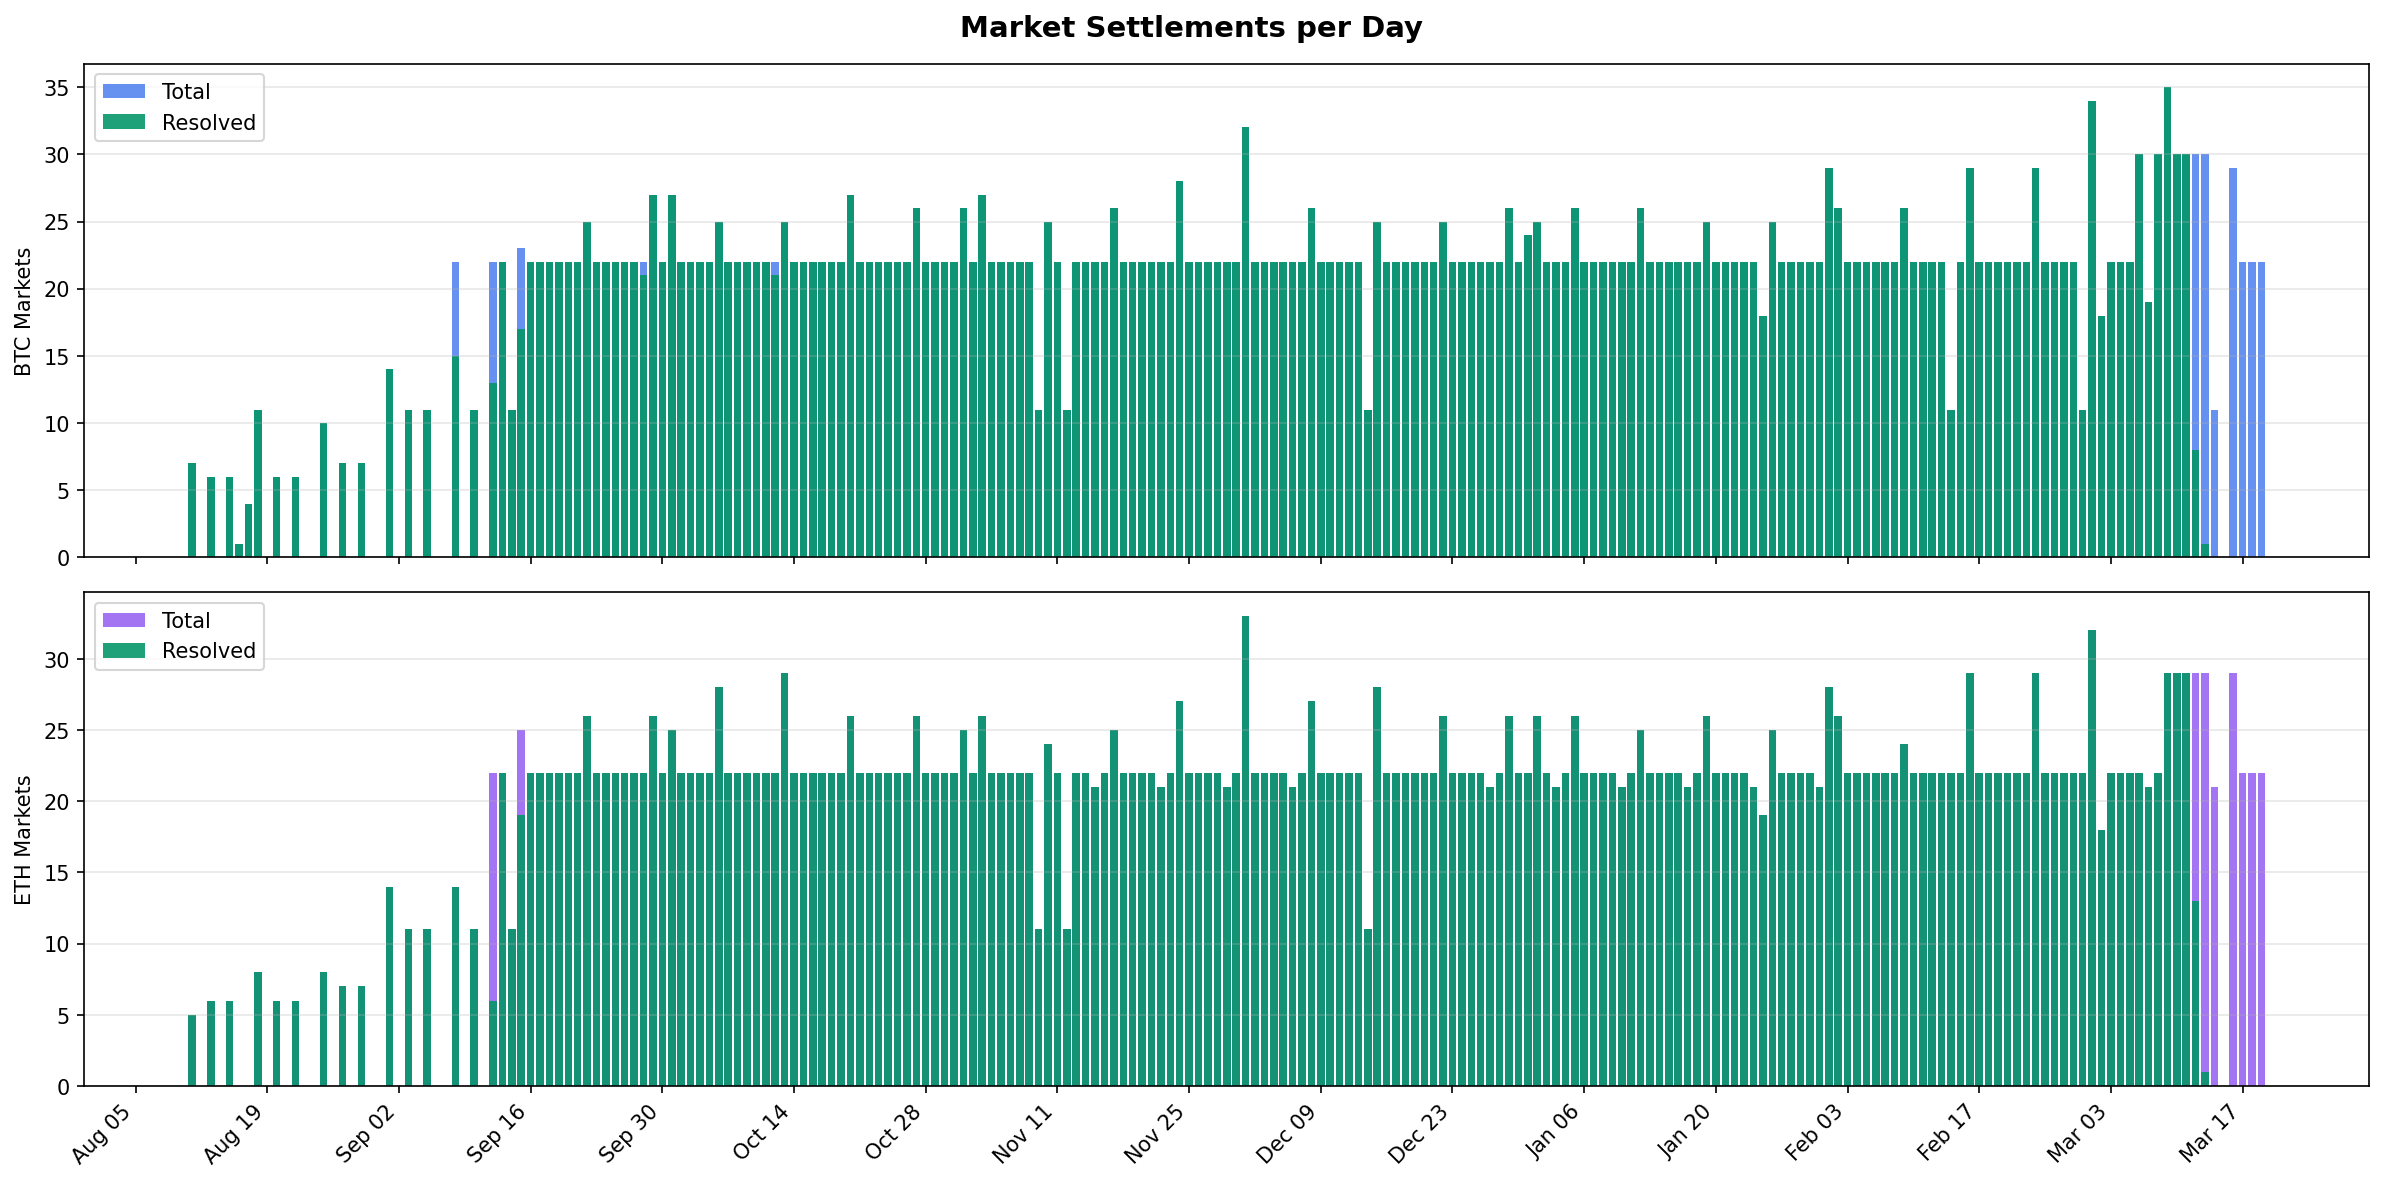
\includegraphics[width=\linewidth]{01_settlements_per_day.png}\\[-2pt]
{\small (a) Daily settlements}
\end{minipage}\hfill
\begin{minipage}[t]{0.31\linewidth}
\centering
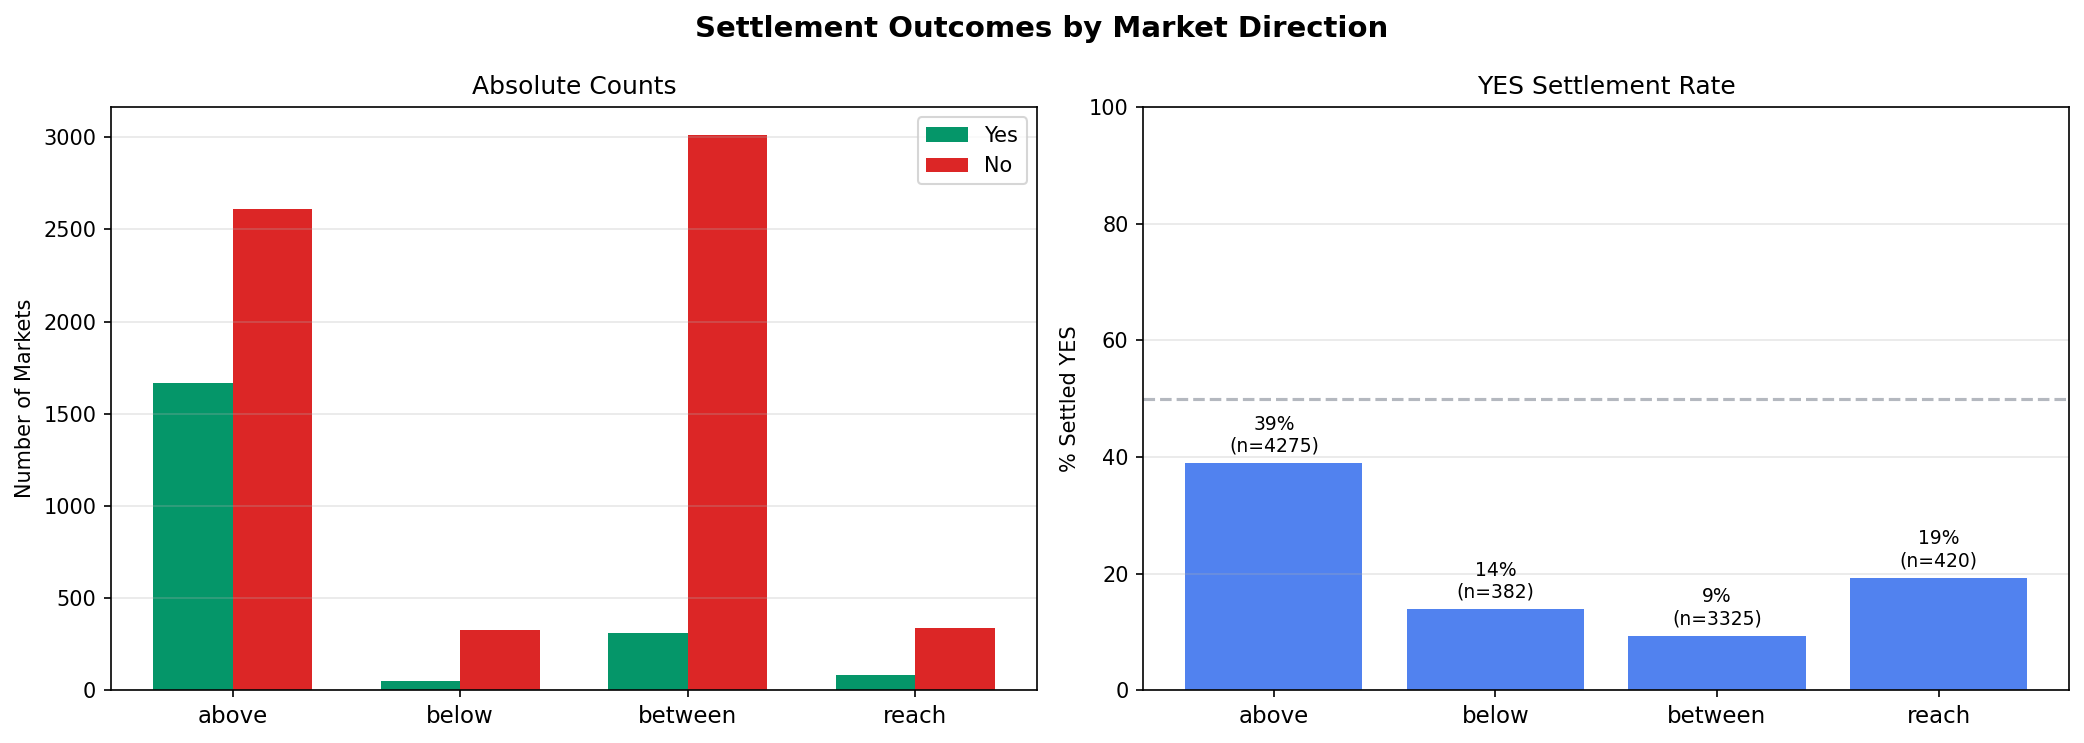
\includegraphics[width=\linewidth]{04_outcome_distribution.png}\\[-2pt]
{\small (b) Outcome distribution}
\end{minipage}\hfill
\begin{minipage}[t]{0.31\linewidth}
\centering
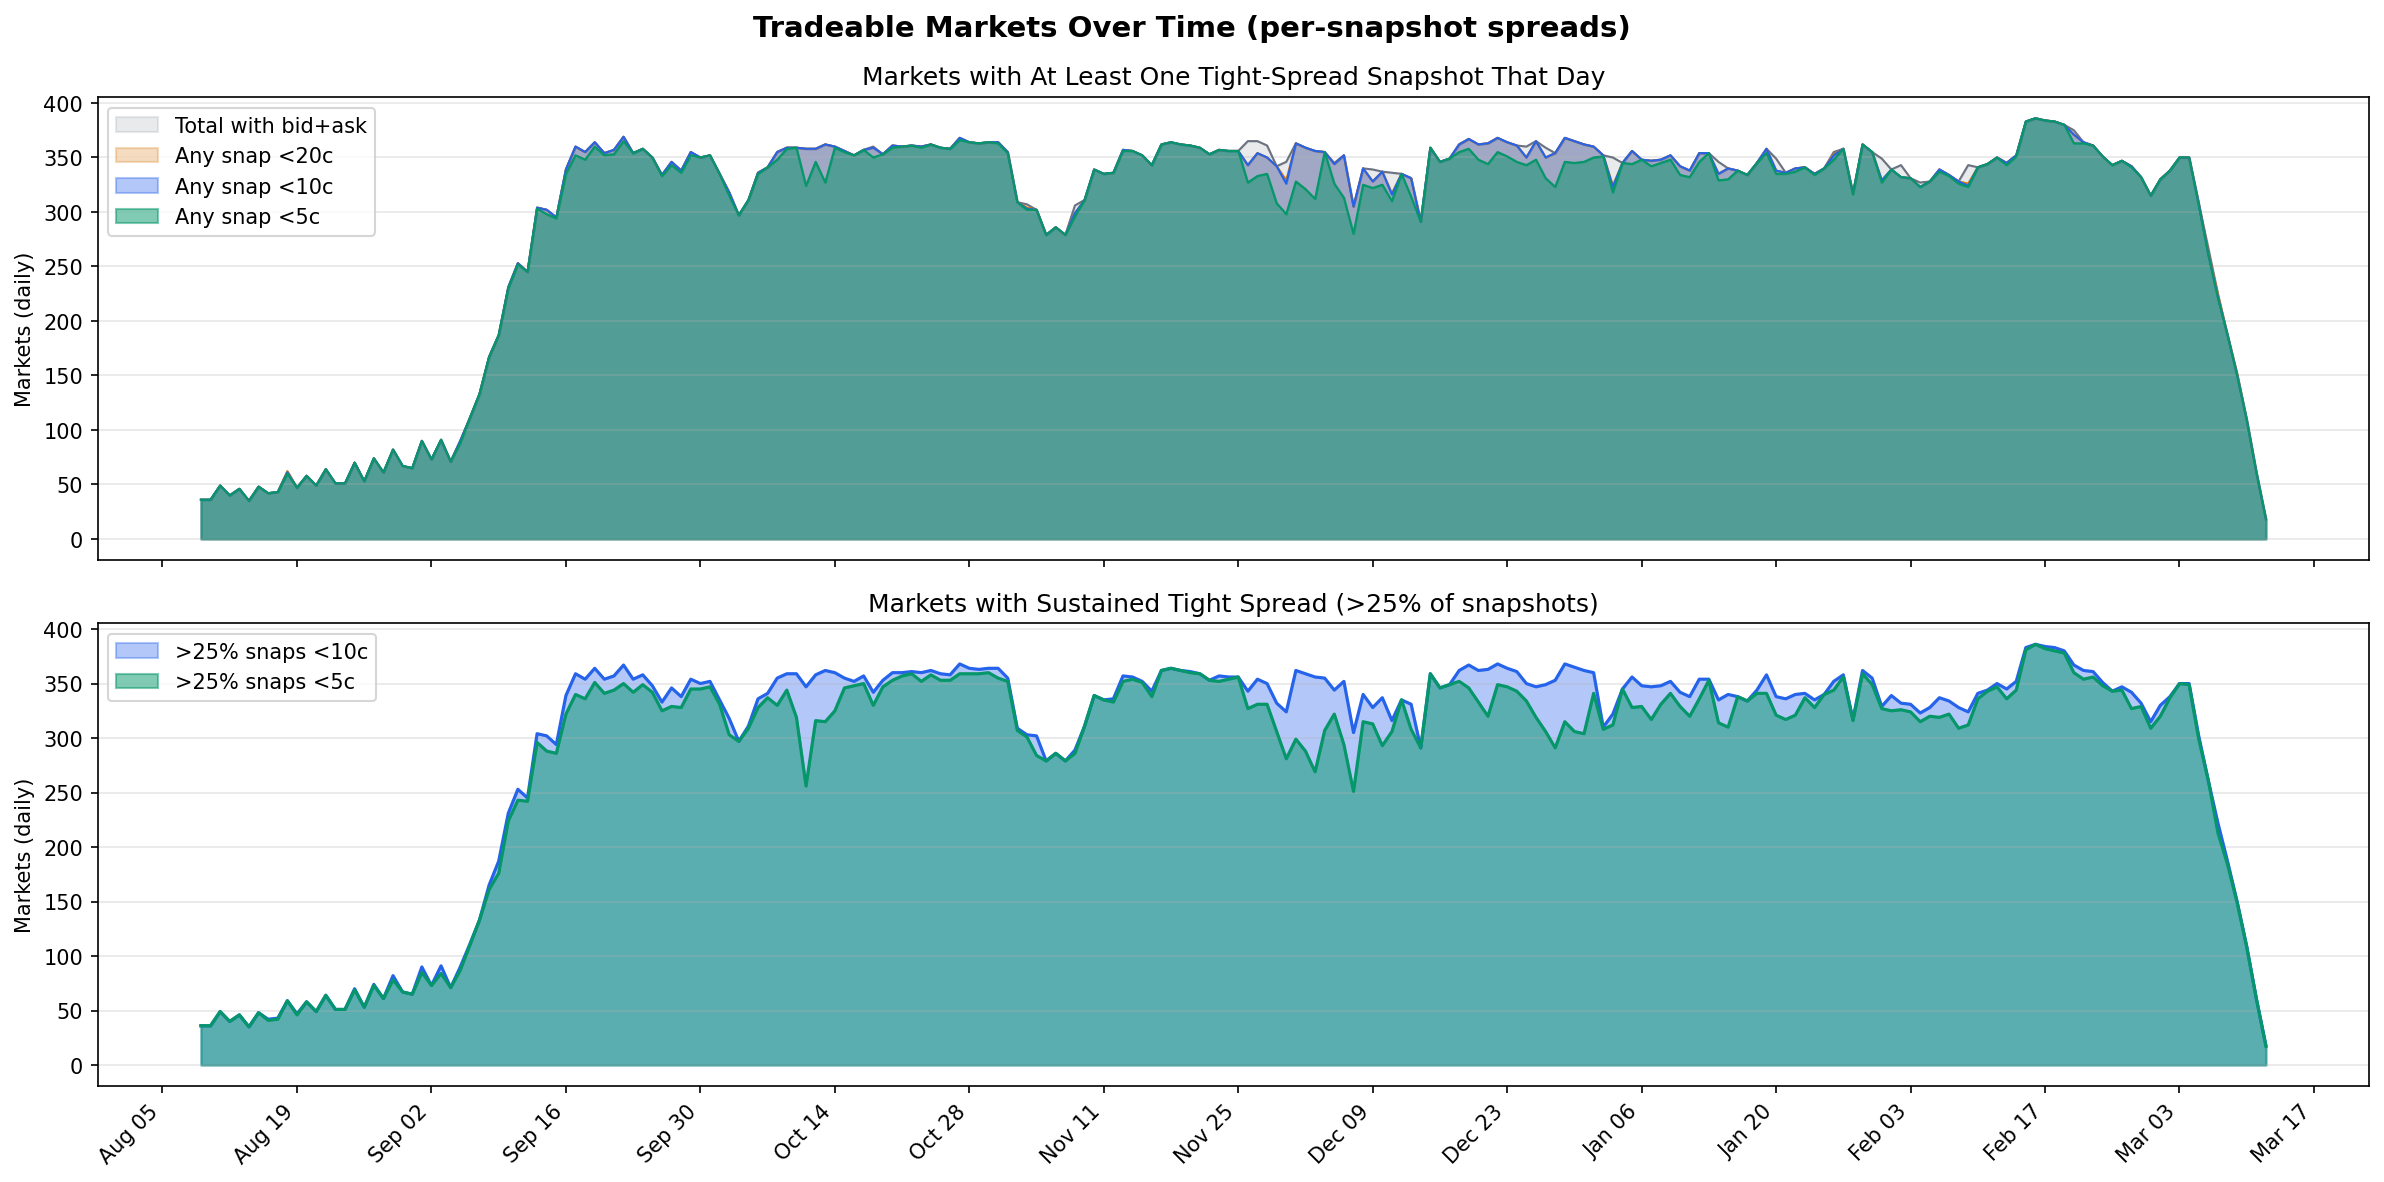
\includegraphics[width=\linewidth]{06_tradeable_markets_over_time.png}\\[-2pt]
{\small (c) Tradeable markets}
\end{minipage}

\vspace{4pt}

\begin{minipage}[t]{0.31\linewidth}
\centering
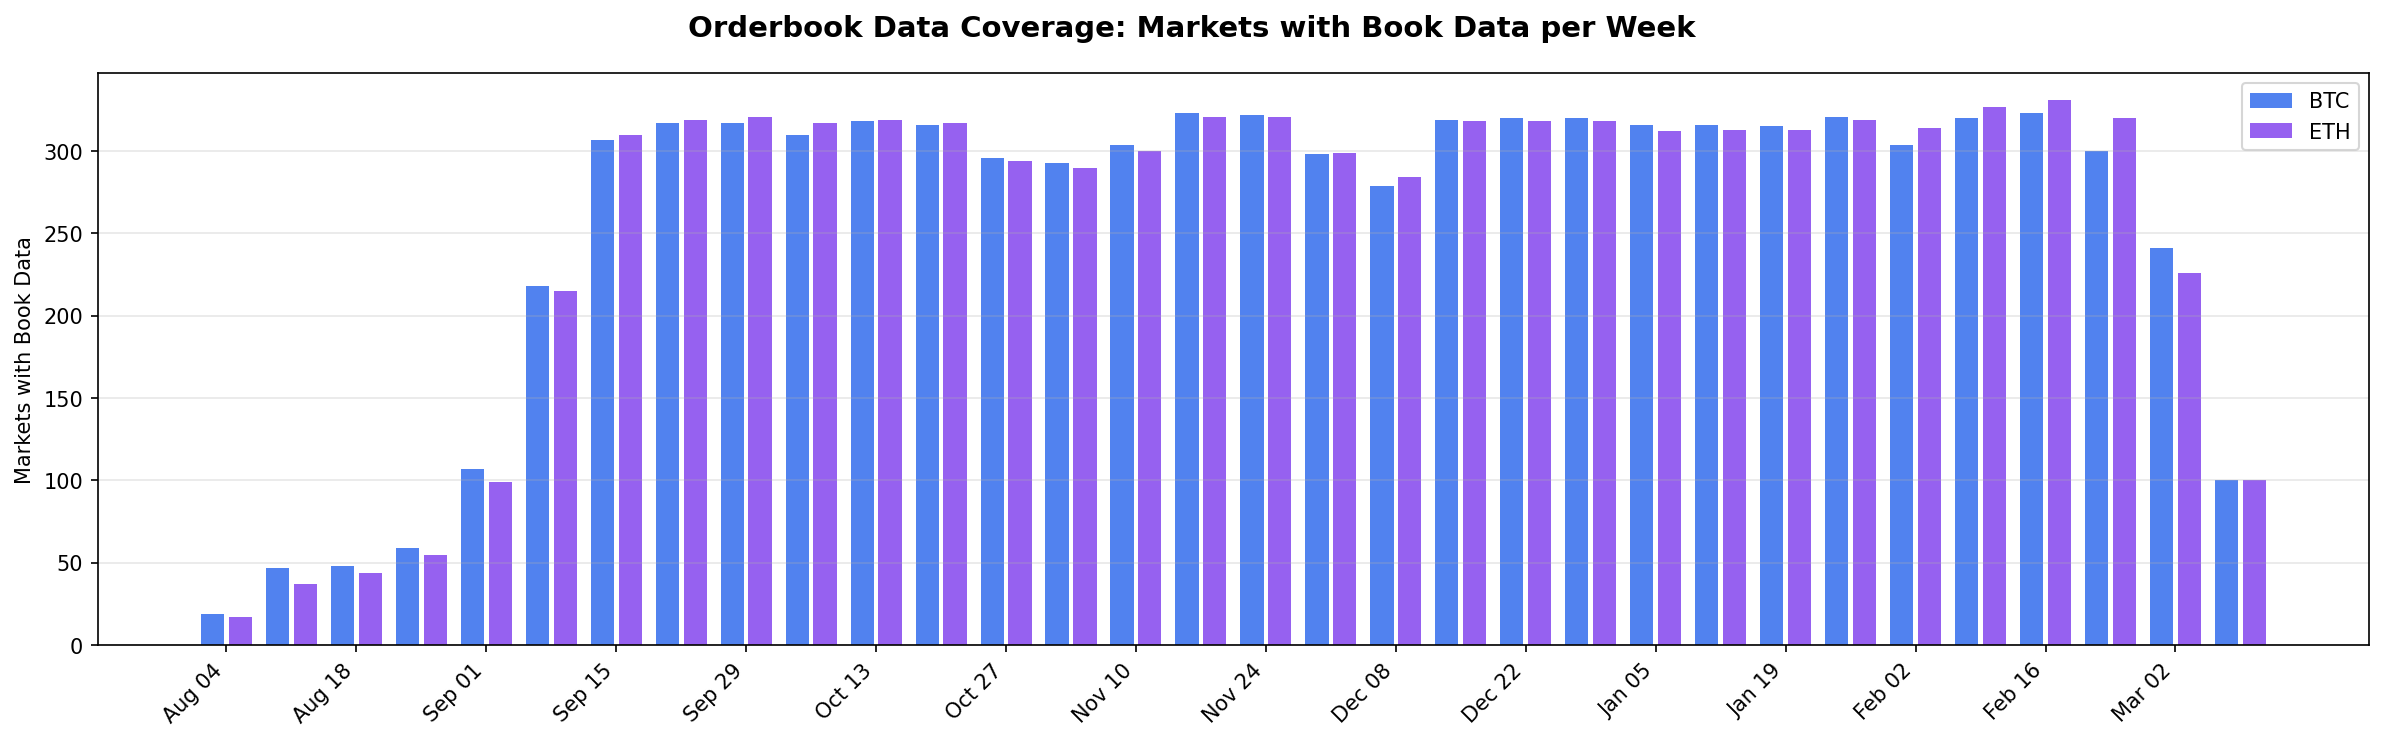
\includegraphics[width=\linewidth]{02_book_coverage_by_week.png}\\[-2pt]
{\small (d) Book coverage by week}
\end{minipage}\hfill
\begin{minipage}[t]{0.31\linewidth}
\centering
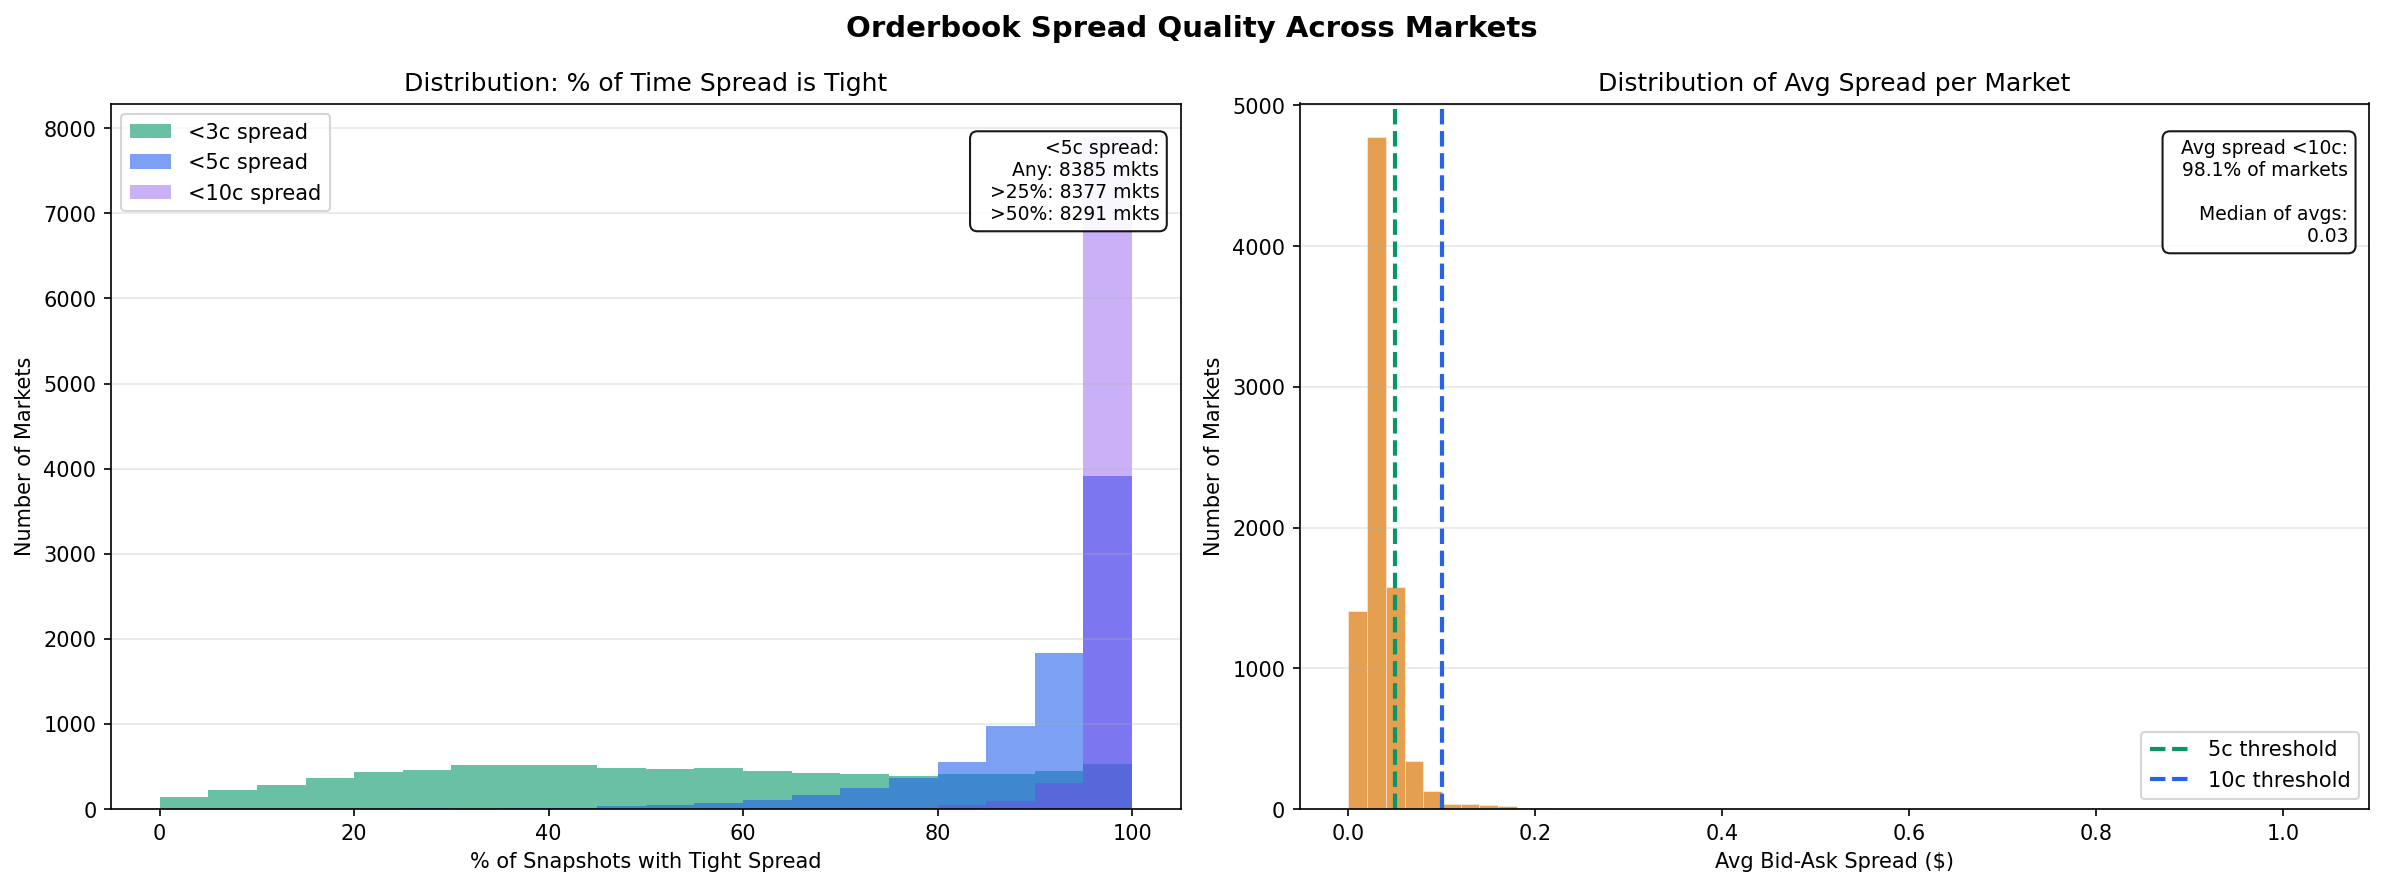
\includegraphics[width=\linewidth]{03_spread_quality.png}\\[-2pt]
{\small (e) Bid-ask spread distribution}
\end{minipage}\hfill
\begin{minipage}[t]{0.31\linewidth}
\centering
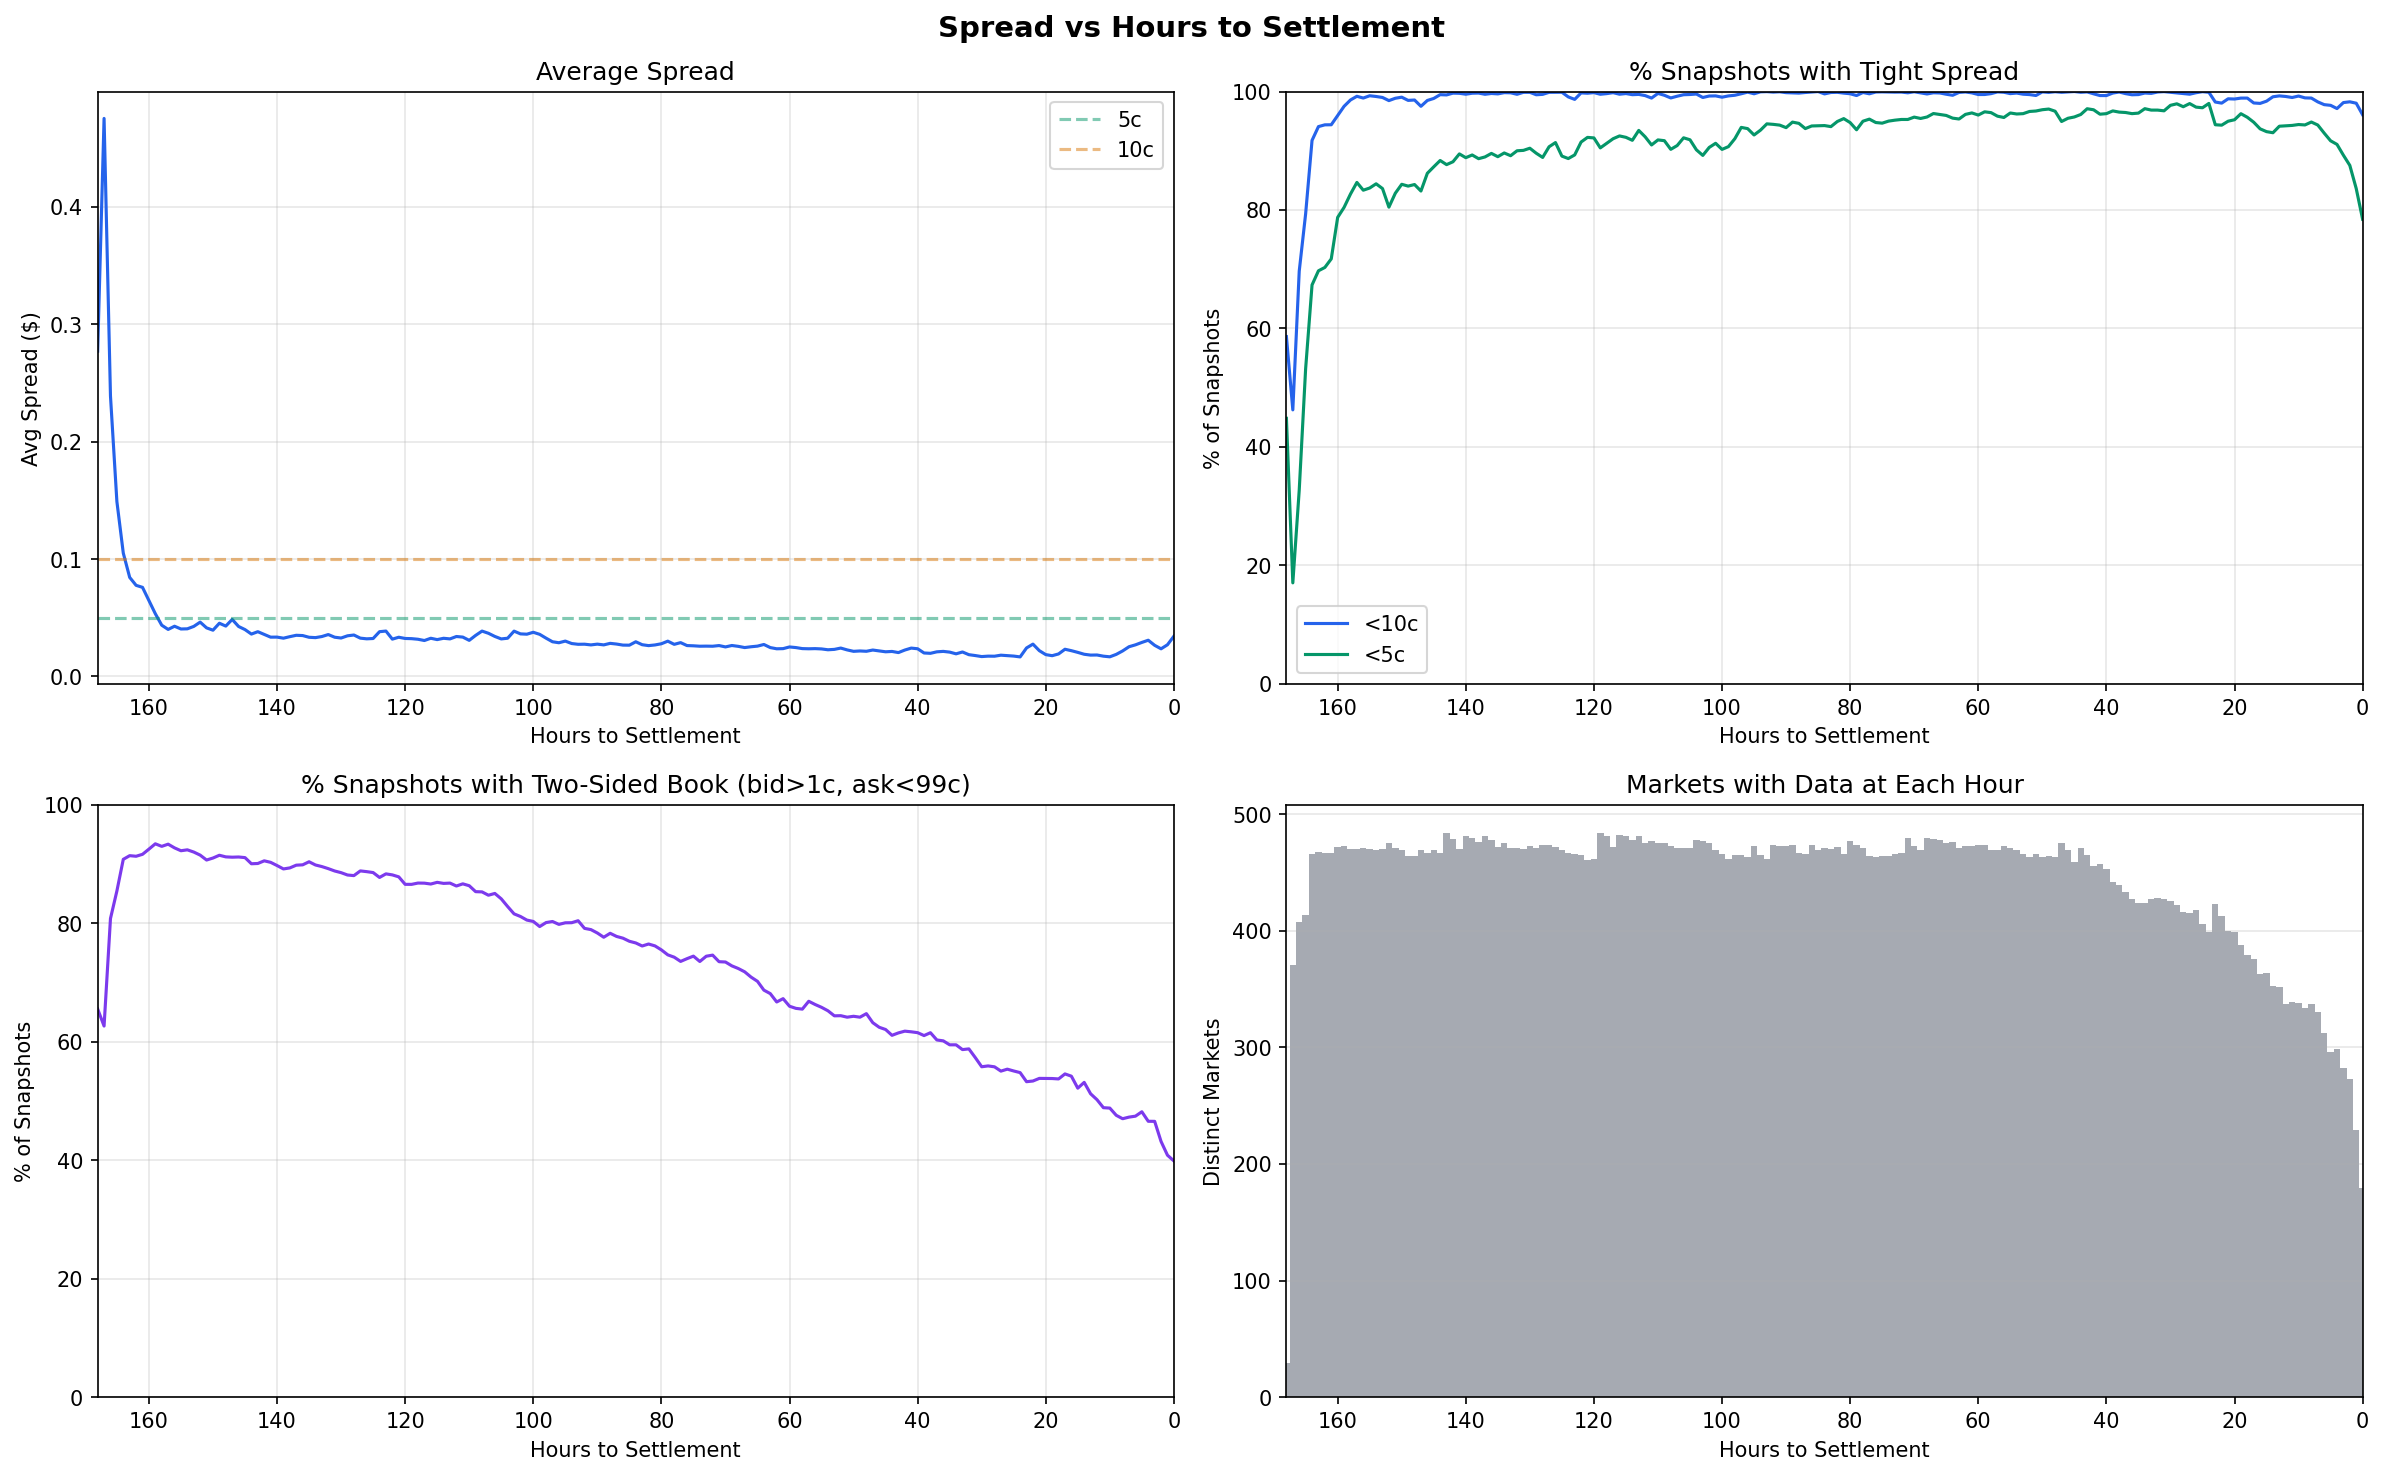
\includegraphics[width=\linewidth]{08_spread_near_settlement.png}\\[-2pt]
{\small (f) Spread near settlement}
\end{minipage}

\caption{Overview of the Polymarket BTC/ETH dataset (April 2025 -- February 2026). Settlement volume is concentrated on the daily cohort (a); the contract mix is dominated by \emph{above} markets, most of which resolve No (b). Tradeable-market counts (c) and weekly book coverage (d) confirm the dataset is fully populated across the full window. Spreads (e) are tight at the median and tighten further as markets approach settlement (f).}
\label{fig:data}
\end{figure}

\begin{table}[t]
\caption{Canonical schema produced by the SQLite adapter.}
\label{tab:schema}
\begin{center}
\small
\begin{tabular}{@{}lll@{}}
\toprule
\textbf{Table} & \textbf{Columns} & \textbf{Source} \\
\midrule
\texttt{markets}      & \texttt{market\_id, asset, contract\_type,}                                & \texttt{markets} \\
                       & \texttt{strike, settlement\_time, label}                                   & \\
\texttt{observations} & \texttt{market\_id, timestamp, mid\_price,}                                & \texttt{market\_prices} \\
                       & \texttt{spread, liquidity, volume, reference\_spot\_price}                 & $\bowtie$ \texttt{ohlcv} \\
\bottomrule
\end{tabular}
\end{center}
\end{table}

\subsection{Snapshot Construction}

For each market $m$ we keep the \emph{latest} observation with $t \le \tau_m = T_m - 24\text{h}$. Markets without an eligible observation are dropped, as are markets without a matching hourly spot anchor. After this filter $4{,}081$ markets remain across $397$ cohorts (BTC: $2{,}047$, ETH: $2{,}034$); the median snapshot is $1$ hour stale relative to $\tau_m$, with the $75$\textsuperscript{th} percentile at $3$ hours. The snapshot vector contains the crowd probability $p_m^{\text{crowd}} = \texttt{mid\_price}_m$, the no-arbitrage spread, raw liquidity and trade-count features, and the signed strike-to-spot distance $\delta_m = (K_m - S_{\tau_m})/S_{\tau_m}$.

\subsection{Cohort Similarity Graphs}

For every cohort $\mathcal{C} \in \mathcal{C}_{a,t}$ we build an undirected weighted graph $G_\mathcal{C} = (V_\mathcal{C}, E_\mathcal{C}, w)$ whose nodes are the markets in $\mathcal{C}$. The weight on edge $(i,j)$ combines two cosine-style similarities:
\begin{equation}
\mathrm{sim}_{\text{strike}}(i,j) = \exp\!\left(-\frac{|\,|\delta_i| - |\delta_j|\,|}{\sigma_K}\right),
\qquad
\mathrm{sim}_{\text{traj}}(i,j) = \tfrac{1}{2}\!\left(1 + \rho\bigl(\tilde{p}_i, \tilde{p}_j\bigr)\right),
\end{equation}
where $\sigma_K = 0.10$ controls the strike kernel bandwidth, $\tilde{p}_m$ is the standardised mid-price trajectory over the last $L=8$ observations within $\tau_m - 72\text{h}$, and $\rho$ is Pearson correlation. The edge weight is the convex combination
\begin{equation}
w(i,j) = \alpha\,\mathrm{sim}_{\text{strike}}(i,j) + (1-\alpha)\,\mathrm{sim}_{\text{traj}}(i,j), \quad \alpha = 0.65,
\end{equation}
and edges with $w(i,j) < 0.25$ are pruned. Figure~\ref{fig:cohort} shows a representative cohort graph; nodes carry the market's strike and contract type as labels and the crowd probability as colour.

\begin{figure}[t]
\centering
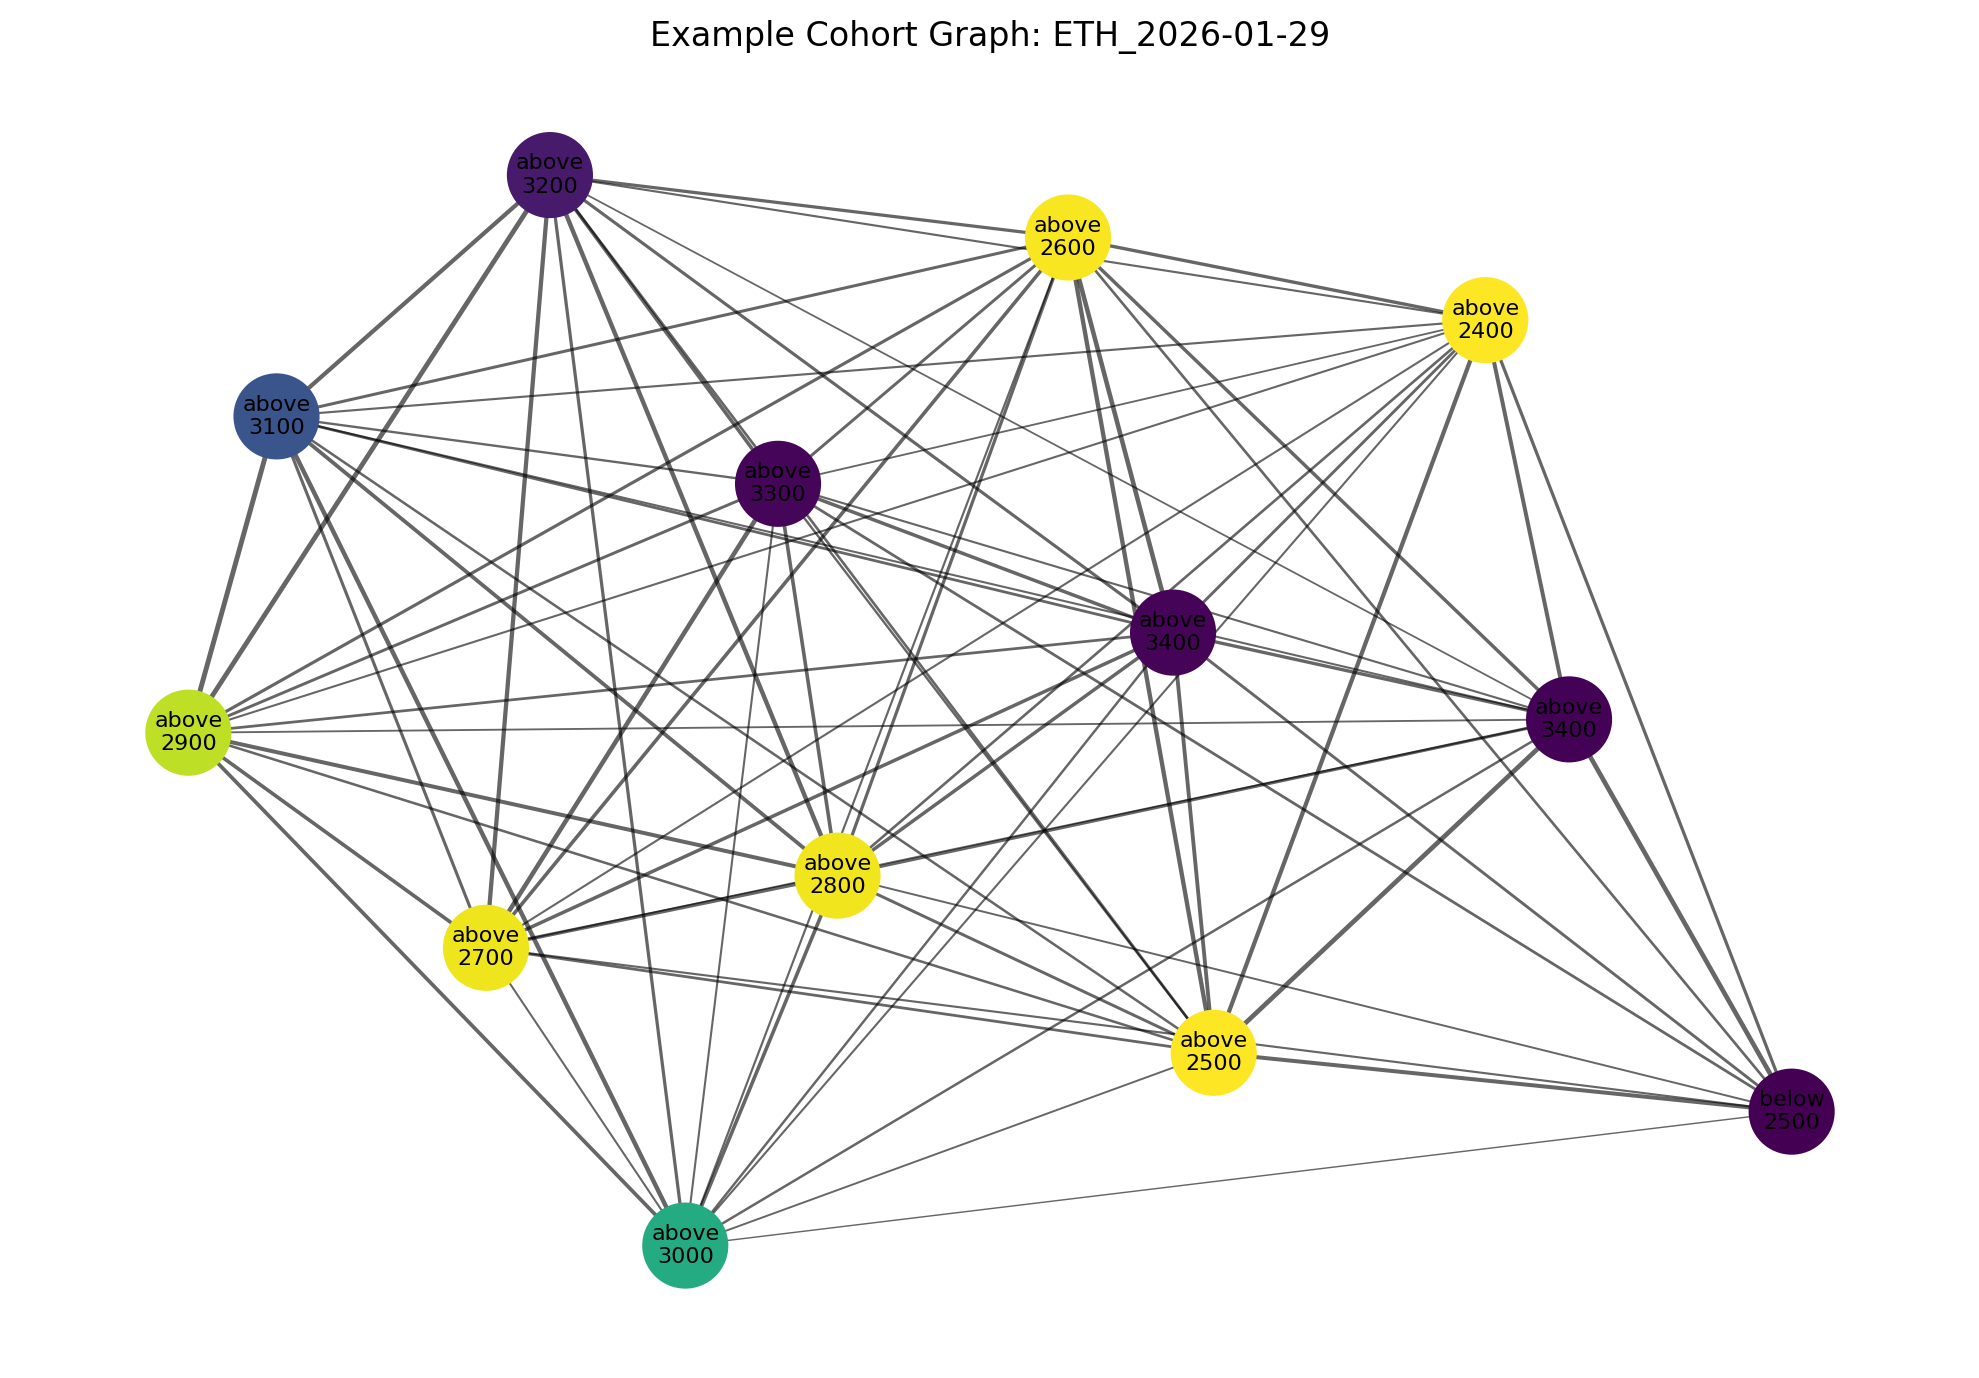
\includegraphics[width=0.78\linewidth]{example_cohort_graph.png}
\caption{Example cohort graph for one BTC settlement day. Each node is a market in the cohort (label: \texttt{contract\_type} and strike); colour encodes the crowd probability and edge width is the similarity weight $w(i,j)$.}
\label{fig:cohort}
\end{figure}

\subsection{Graph Features}

\textbf{Centrality features.} Per node we extract weighted degree $\sum_j w(i,j)$, weighted clustering coefficient, weighted PageRank, and weighted neighbour means of the crowd probability, liquidity, and spread (six features in total).

\textbf{\texttt{node2vec} embeddings.} We assemble the union graph $G^\star = \bigsqcup_\mathcal{C} G_\mathcal{C}$ over all cohorts. By construction, cohorts are disjoint connected components of $G^\star$, so biased random walks cannot cross from one cohort into another --- the union construction therefore preserves the leakage constraint while letting one Skip-gram model see a much larger corpus than per-cohort fits would. We run \texttt{node2vec} \citep{grover2016} with embedding dimension $d=16$, walk length $10$, $40$ walks per source, window size $5$, and default $p=q=1$. Each market $m$ receives an embedding vector $\mathbf{e}_m \in \mathbb{R}^{16}$.

\subsection{Models}

All five comparison models are L2-regularised logistic regressions ($C = 1$) trained on the train cohorts. Numeric features are median-imputed and standardised; categorical features (\texttt{asset}, \texttt{contract\_type}) are one-hot encoded. The base feature set $\mathcal{F}_{\text{tab}}$ is $\{p^{\text{crowd}}, \texttt{spread}, \texttt{liquidity}, \texttt{volume}, \delta\}$. The five models differ only in which graph features they add:
\begin{enumerate}[leftmargin=*,itemsep=2pt,topsep=2pt]
\item \textbf{Crowd baseline} --- raw $p^{\text{crowd}}$ clipped to $[10^{-6}, 1-10^{-6}]$, no learning.
\item \textbf{Tabular} --- $\mathcal{F}_{\text{tab}}$.
\item \textbf{Graph (centrality)} --- $\mathcal{F}_{\text{tab}} \cup \{$ six centrality features $\}$.
\item \textbf{Graph (\texttt{node2vec})} --- $\mathcal{F}_{\text{tab}} \cup \{e_m^{(1)}, \dots, e_m^{(16)}\}$.
\item \textbf{Graph (combined)} --- $\mathcal{F}_{\text{tab}} \cup \{$ centrality $\} \cup \{$ embedding $\}$.
\end{enumerate}

\subsection{Limitations and Implementation Notes}

Three implementation choices deserve flagging as deviations from the proposal. First, the trajectory similarity is computed over raw standardised mid-prices rather than residualised returns; we believe the cohort-internal restriction prevents the dominant spot factor from propagating across the train/test boundary, but a residualised variant remains the cleaner construction. Second, the \texttt{node2vec} fit is static --- a single model on the union graph --- whereas the proposal envisages a dynamic, observation-window-conditioned fit. Third, hourly OHLCV is used as the spot anchor (\textsc{ms} timestamps, joined on the snapshot's hour-floor); this is sufficient for the $24$-hour horizon but loses sub-hour resolution.

% ============================================================
\section{Evaluation}
% ============================================================

\subsection{Experimental Protocol}

Cohorts are sorted chronologically by their settlement date and partitioned $60$/$20$/$20$ at the cohort level: $238$ train cohorts ($2{,}047$ markets), $79$ validation cohorts ($1{,}002$), and $80$ test cohorts ($1{,}032$). Two automated invariants are checked at the end of every pipeline run: every cohort appears in exactly one split, and every snapshot is exactly $24$ hours before its market's settlement, with no observation later than the snapshot. The embedding fit and all logistic regressions are seeded ($\texttt{seed}=42$) for reproducibility.

\subsection{Headline Results}

Table~\ref{tab:test} reports per-model performance on the test cohorts, sorted by Brier score. The \texttt{node2vec} model wins on Brier and log-loss with sizeable margins over the crowd baseline ($-8.1\%$ Brier, $-9.4\%$ log-loss), while classical centrality features added on top of the tabular baseline produce no measurable improvement. The combined model essentially replicates \texttt{node2vec}, suggesting the embedding already absorbs the structural signal that the centrality features would carry.

\begin{table}[t]
\caption{Test-split metrics (1{,}032 markets), sorted by Brier score.}
\label{tab:test}
\begin{center}
\small
\begin{tabular}{@{}lrrrr@{}}
\toprule
\textbf{Model} & \textbf{$n$} & \textbf{Brier} $\downarrow$ & \textbf{Log-loss} $\downarrow$ & \textbf{ECE} $\downarrow$ \\
\midrule
Graph (\texttt{node2vec})  & 1{,}032 & \textbf{0.0542} & \textbf{0.1898} & 0.0324 \\
Graph (combined)           & 1{,}032 & 0.0543 & 0.1900 & 0.0339 \\
Tabular                    & 1{,}032 & 0.0569 & 0.1966 & \textbf{0.0181} \\
Graph (centrality)         & 1{,}032 & 0.0574 & 0.1978 & 0.0241 \\
Crowd baseline             & 1{,}032 & 0.0590 & 0.2094 & 0.0310 \\
\bottomrule
\end{tabular}
\end{center}
\end{table}

\begin{figure}[t]
\centering
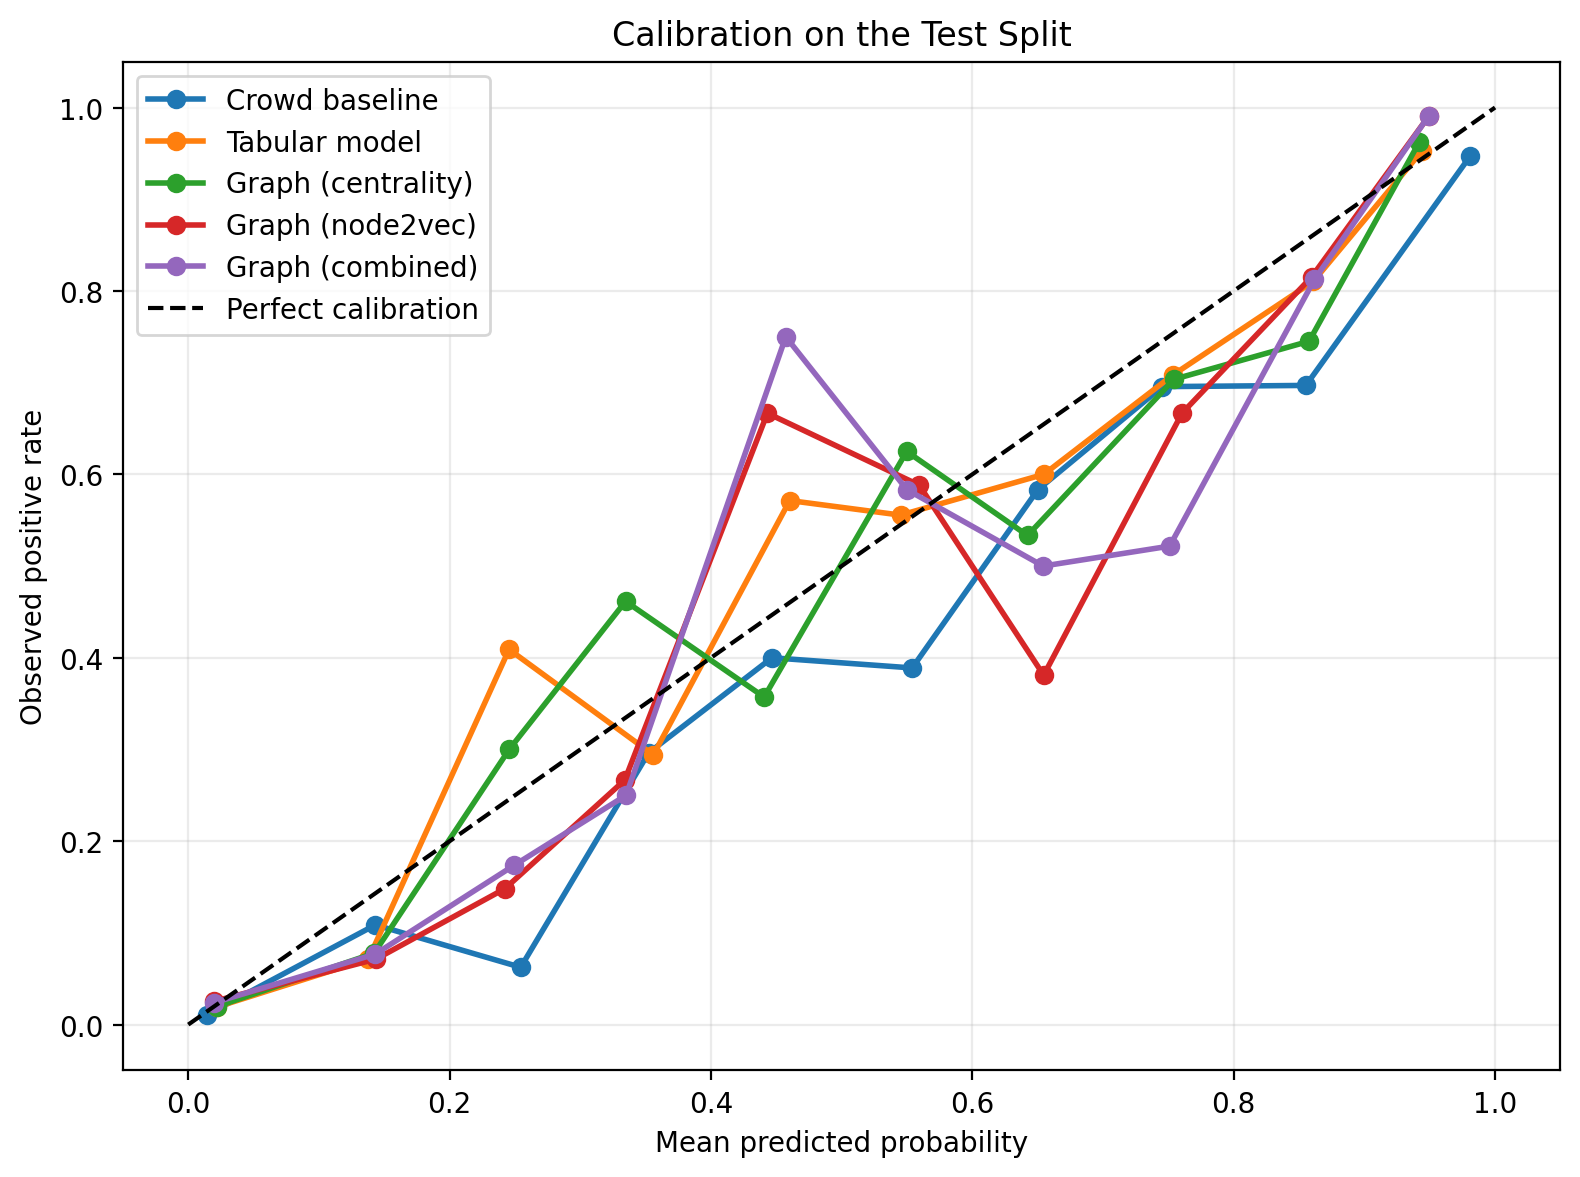
\includegraphics[width=0.72\linewidth]{calibration_plot.png}
\caption{Reliability diagrams for all five models on the test split. The diagonal is perfect calibration. The tabular model is best calibrated at the extremes; the embedding model is more discriminative but slightly miscalibrated.}
\label{fig:calibration}
\end{figure}

\subsection{Per-Split Behaviour and the Validation Anomaly}

Table~\ref{tab:per-split} extends the comparison to all three splits. Two observations matter. First, the train-split Brier of every learned model is meaningfully below its test-split Brier, but the \emph{ranking} on train is the same as on test --- the models that win in-sample also win out-of-sample. Second, on validation the order \emph{inverts}: the crowd baseline is the best model and every learned variant is worse. This is not a small effect ($0.0502$ vs $0.0603$ Brier for the embedding model). The validation cohorts cover August--October 2025, a window in which YES outcomes resolved at $43\%$ versus $\sim 33\%$ on either side --- the spot drifted in a direction that lined up with the dominant \emph{above} questions, and the crowd appears to have priced this regime unusually well, leaving little residual for any model to capture. The fact that the same \texttt{node2vec} features that hurt on validation help on test (the more dispersive November 2025 -- February 2026 window) suggests graph-derived signal is most useful precisely when the crowd is \emph{not} already perfectly calibrated. We see this as evidence that the embedding does not learn a generic ``constant edge'' over the crowd, but rather a state-contingent correction --- a desirable property for a research method, even if it makes the validation-set metric a poor model-selection signal here.

\begin{table}[t]
\caption{All-split Brier / log-loss / ECE per model.}
\label{tab:per-split}
\begin{center}
\small
\begin{tabular}{@{}llrrr@{}}
\toprule
\textbf{Split} & \textbf{Model} & \textbf{Brier} & \textbf{Log-loss} & \textbf{ECE} \\
\midrule
Train      & Crowd baseline             & 0.0793 & 0.2568 & 0.0341 \\
Train      & Tabular                    & 0.0781 & 0.2565 & 0.0228 \\
Train      & Graph (centrality)         & 0.0774 & 0.2542 & 0.0254 \\
Train      & Graph (\texttt{node2vec})  & 0.0733 & 0.2434 & 0.0155 \\
Train      & Graph (combined)           & 0.0728 & 0.2418 & 0.0171 \\
\midrule
Validation & Crowd baseline             & 0.0502 & 0.1658 & 0.0168 \\
Validation & Tabular                    & 0.0553 & 0.1984 & 0.0347 \\
Validation & Graph (centrality)         & 0.0555 & 0.1995 & 0.0395 \\
Validation & Graph (\texttt{node2vec})  & 0.0603 & 0.2168 & 0.0299 \\
Validation & Graph (combined)           & 0.0605 & 0.2172 & 0.0275 \\
\midrule
Test       & Crowd baseline             & 0.0590 & 0.2094 & 0.0310 \\
Test       & Tabular                    & 0.0569 & 0.1966 & 0.0181 \\
Test       & Graph (centrality)         & 0.0574 & 0.1978 & 0.0241 \\
Test       & Graph (\texttt{node2vec})  & 0.0542 & 0.1898 & 0.0324 \\
Test       & Graph (combined)           & 0.0543 & 0.1900 & 0.0339 \\
\bottomrule
\end{tabular}
\end{center}
\end{table}

\subsection{Calibration vs Discrimination}

Figure~\ref{fig:calibration} plots reliability diagrams for the five models on the test split. The tabular logistic regression is the most calibrated near the extremes (lowest ECE, $0.0181$), while the embedding model trades a small amount of calibration ($\text{ECE}=0.0324$) for noticeably sharper probabilities and the lower Brier. This is consistent with the fact that the embedding pushes the predictive distribution away from the prior more aggressively than the tabular model does. A natural fix --- isotonic recalibration on validation, then re-evaluation on test --- would likely close the ECE gap and is the most obvious follow-up; we leave it for future work because honest cross-validated isotonic on a chronological split would require splitting the validation set further, and the validation-anomaly above suggests that any recalibration learned on August--October 2025 may not transfer to the test window.

\subsection{Ablation: What Carries the Signal?}

The four learned models in Table~\ref{tab:test} form a $2\times 2$ ablation: classical centrality features in $\{$on, off$\}$ $\times$ \texttt{node2vec} embedding in $\{$on, off$\}$. The interaction is striking: turning centrality on alone (Graph-centrality vs Tabular) costs $0.0005$ Brier on test; turning the embedding on alone (Graph-\texttt{node2vec} vs Tabular) gains $0.0027$; turning both on (Graph-combined) gains the same $0.0026$ as the embedding alone. We conclude that within-cohort centrality, when added to a tabular feature set that already contains the strike-to-spot distance, provides essentially no independent information --- this makes intuitive sense, because in our construction the dominant ingredient of every weight is strike proximity, which is precisely what the strike-to-spot distance already encodes. The \texttt{node2vec} embedding, by contrast, jointly summarises strike proximity, trajectory similarity, and global cohort position into $16$ continuous coordinates that the linear classifier can mix flexibly.

% ============================================================
\section{Conclusions and Future Work}
% ============================================================

We set out to test whether graph structure between same-day Polymarket binary contracts adds probabilistic information beyond the crowd-implied price. On $4{,}081$ resolved BTC and ETH markets settled between April 2025 and February 2026, evaluated under a leakage-safe chronological cohort split, the answer is yes --- but only when the structure is encoded as a learned \texttt{node2vec} embedding. The embedding model cuts test Brier by $8.1\%$ and log-loss by $9.4\%$ relative to the crowd baseline, while classical centrality features alone do not improve over a tabular microstructure logistic regression. The improvement is robust to the addition of centrality on top of the embedding (no interaction) and survives a strong validation-set anomaly that would have rejected the model under naive validation-driven model selection.

The most promising extensions follow the limitations flagged in Section~\ref{sec:methodology}. (1) Replace the trajectory similarity with one based on residualised returns (regress out the cohort-asset's hour-by-hour spot move first); this should make the graph signal demonstrably independent of crude spot proximity. (2) Replace the static union-graph \texttt{node2vec} with an observation-conditioned dynamic model --- a temporal GCN or a streaming embedding --- that lets the embedding evolve as new ticks arrive within the snapshot window. (3) Add isotonic recalibration on a held-out portion of training cohorts to recover the calibration loss; combined with (2), this would target both the ECE gap and the validation regime-shift weakness. (4) Broaden the contract universe beyond \emph{above}/\emph{below} (currently $90\%/10\%$ in our filter) to include \emph{between}, \emph{reach}, and \emph{dip} markets, which would test whether the graph signal generalises beyond European digital structures.

% ============================================================
% References
% ============================================================

\begin{thebibliography}{10}

\bibitem[Boginski et al.(2005)]{boginski2005} V. Boginski, S. Butenko, and P.M. Pardalos. Statistical analysis of financial networks. \textit{Comput. Stat. Data Anal.}, 48(2):431--443, 2005.

\bibitem[Chen et al.(2018)]{chen2018} Y. Chen, Z. Wei, and X. Huang. Incorporating corporation relationship via graph convolutional neural networks for stock price prediction. In \textit{CIKM}, pp.\ 1655--1658, 2018.

\bibitem[Fenn et al.(2012)]{fenn2012} D.J. Fenn, M.A. Porter, P.J. Mucha, M. McDonald, S. Williams, N.F. Johnson, and N.S. Jones. Dynamical clustering of exchange rates. \textit{Quant. Finance}, 12(10):1493--1520, 2012.

\bibitem[Grover \& Leskovec(2016)]{grover2016} A. Grover and J. Leskovec. node2vec: Scalable feature learning for networks. In \textit{KDD}, pp.\ 855--864, 2016.

\bibitem[Isogai(2017)]{isogai2017} T. Isogai. Dynamic correlation network analysis of financial asset returns with network clustering. \textit{Appl. Netw. Sci.}, 2:8, 2017.

\bibitem[Kipf \& Welling(2017)]{kipf2017} T.N. Kipf and M. Welling. Semi-supervised classification with graph convolutional networks. In \textit{ICLR}, 2017.

\bibitem[Mantegna(1999)]{mantegna1999} R.N. Mantegna. Hierarchical structure in financial markets. \textit{Eur. Phys. J. B}, 11:193--197, 1999.

\bibitem[Onnela et al.(2003)]{onnela2003} J.-P. Onnela, A. Chakraborti, K. Kaski, J. Kert\'{e}sz, and A. Kanto. Dynamics of market correlations: Taxonomy and portfolio analysis. \textit{Phys. Rev. E}, 68(5):056110, 2003.

\bibitem[Wolfers \& Zitzewitz(2004)]{wolfers2004} J. Wolfers and E. Zitzewitz. Prediction markets. \textit{J. Econ. Perspect.}, 18(2):107--126, 2004.

\bibitem[Zhou et al.(2025)]{zhou2025} Y. Zhou, C. Xie, G.-J. Wang, J. Gong, and Y. Zhu. Forecasting cryptocurrency volatility: A novel framework based on the evolving multiscale graph neural network. \textit{Financial Innovation}, 11:87, 2025.

\end{thebibliography}

\end{document}
